\section{Evaluation}
\label{sec:evaluation}

\subsection{Research Questions}

We investigate key research questions to validate the effectiveness and efficiency of \sys:

\begin{itemize}
\item \textbf{RQ1}: Can \sys effectively configure existing schedulers?
\item \textbf{RQ2}: Can \sys generate new schedulers for specific workloads?
\item \textbf{RQ3}: What is the cost and efficiency of \sys's scheduler generation?
\item \textbf{RQ4}: How much can \agent continue to improve performance after initial generation?
% \item \textbf{RQ5}: How effectively can \sys understand workloads?
\end{itemize}

\subsection{Experimental Setup}

We evaluate \sys on an 86-core Intel Xeon 6787P with 758GB RAM, NVMe SSDs, 10Gbps network, running Linux 6.14 with sched\_ext. We test Claude Code (Opus 4) and Gemini-cli (Gemini 2.5 Pro) as AI agents to validate framework generality. For each case, we test 3 times and get the average results.

\subsection{Performance Impact of AI-Driven Optimization}

Figure~\ref{fig:performance-comparison} shows performance improvements across three stages: baseline CFS, LLM-configured schedulers, and Iteration-improved configurations. 

% For schbench, the LLM achieves 50\% lower p99 latency and 30\% higher throughput by selecting scx\_layered. 

The Linux kernel build shows 1.63x speedup from 13.57s to 8.31s using scx\_rusty as the first attemp. After 3 iteration of observe-optimization process, the \agent selects the scx\_layered scheduler and adds 16\% additional gain beyond LLM configuration, with total improvements of 1.79x over baseline CFS.

\begin{figure}[h]
\centering
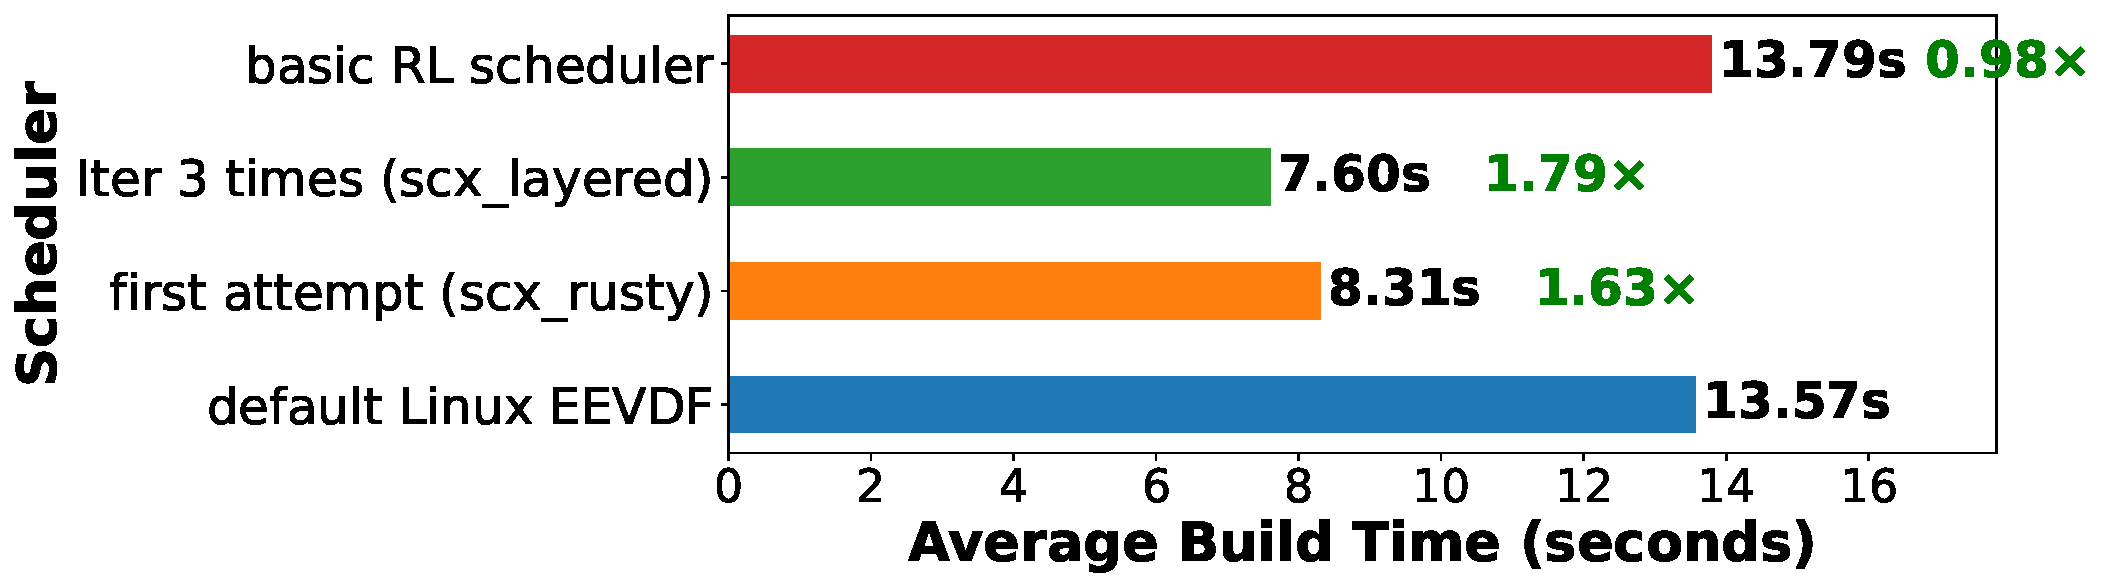
\includegraphics[width=0.9\columnwidth]{sections/Linux_build_benchmark_results.pdf}
\caption{Performance comparison of scheduler configurations with RL improvement showing initial LLM gains (30-80\%) and additional RL improvements (10-12\%).}
\label{fig:performance-comparison}
\end{figure}

\subsection{Scheduler Synthesis for Batch Workloads}

Figure~\ref{fig:batch-performance} demonstrates AI-generated scheduler performance on batch workloads.  Classification cost averages \$0.15 per analysis. We also observed the Agent based on Claude Opus can successfuly classify all the 8 workloads, while sonnet cannot. For unit tests minimizing average wait time, the agent implements SJF scheduling achieving 45\% reduction. For compilation workloads, it implements LJF scheduling with 32\% improvement in makespan. Data analytics workloads see 29\% speedup with a hybrid approach. Claude Opus consistently identifies theoretically optimal strategies, validating the AI's understanding of scheduling principles. .

\begin{figure}[h]
\centering
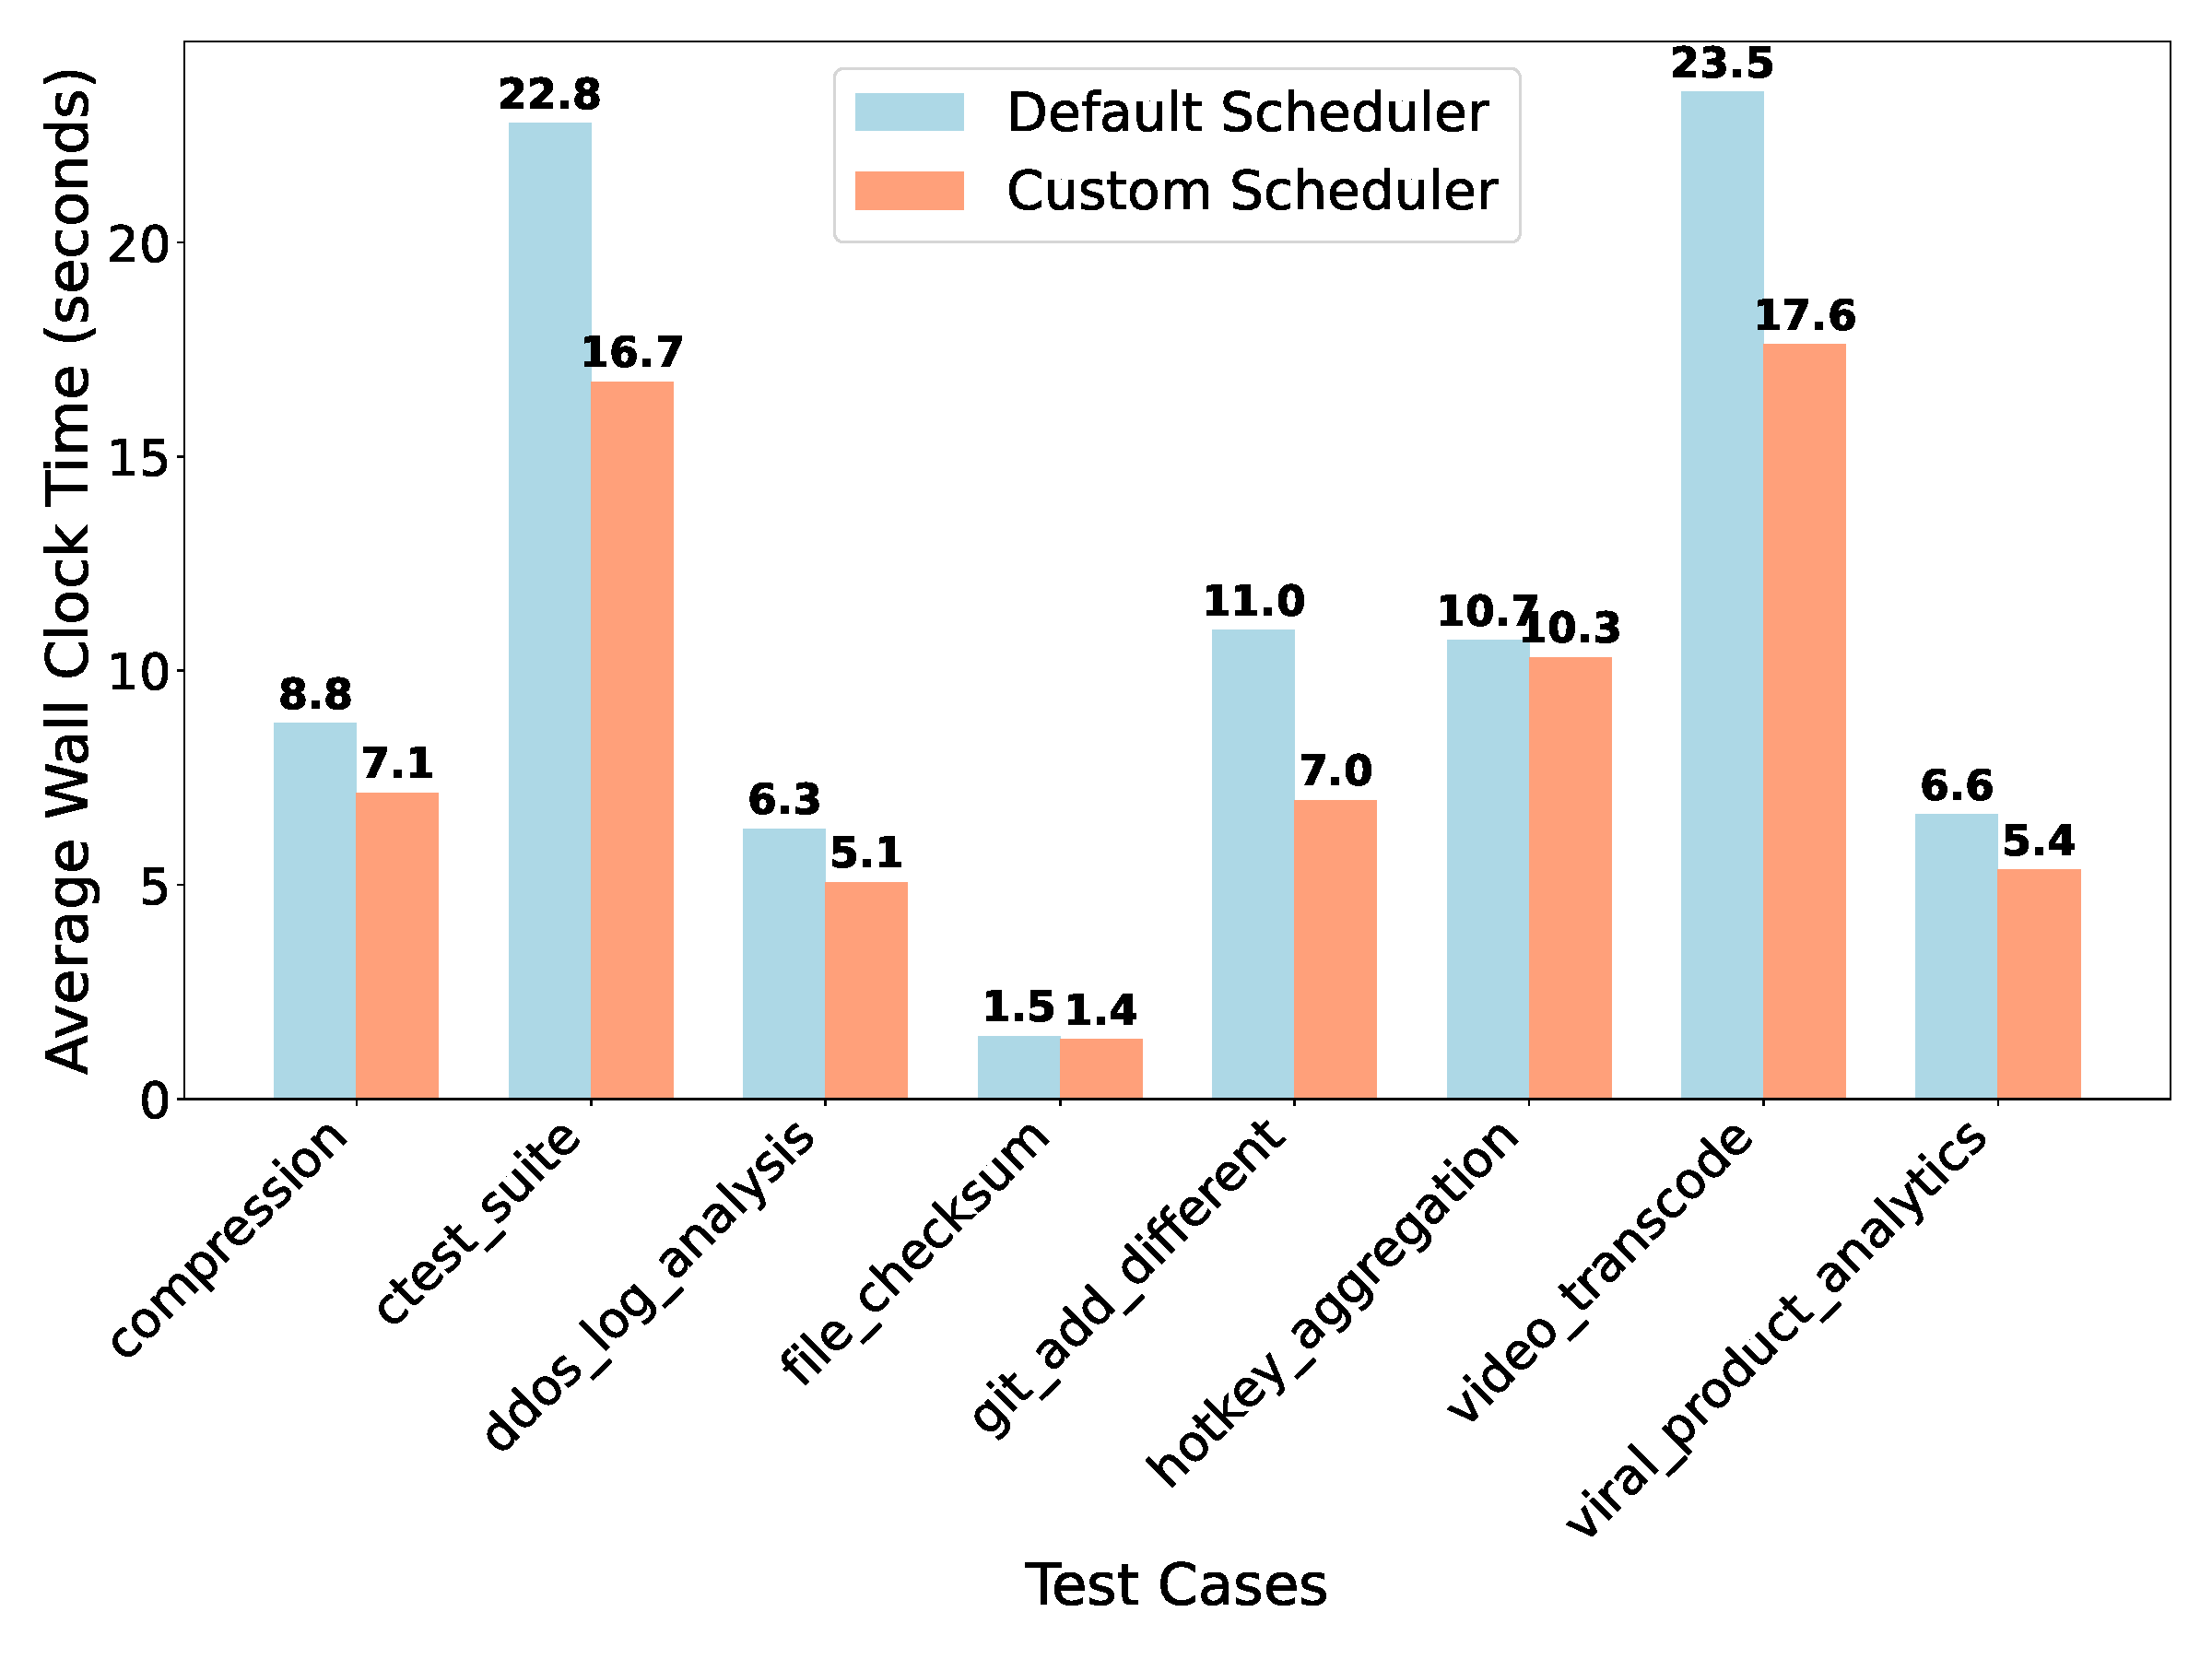
\includegraphics[width=0.9\columnwidth]{sections/scheduler_performance_comparison.pdf}
\caption{AI-generated scheduler performance on batch workloads.}
\label{fig:batch-performance}
\end{figure}

Beyond performance improvements, our framework achieves dramatic cost reductions through systematic optimizations. Generation time drops from 33 minutes to 5 minutes (85\% reduction). API calls decrease from 221 to 28 (87\% reduction). Monetary cost falls from \$6.00 to \$0.75 (88\% reduction). These optimizations make AI-driven scheduler optimization economically viable for production deployment.
